%!TEX TS-program = xelatex
% !TeX spellcheck = de_DE 
\documentclass[11pt]{friggeri-cv}

\begin{document}
\header{Gessica Trivelli}{Hebamme}

% In the aside, each new line forces a line break
\begin{aside}
  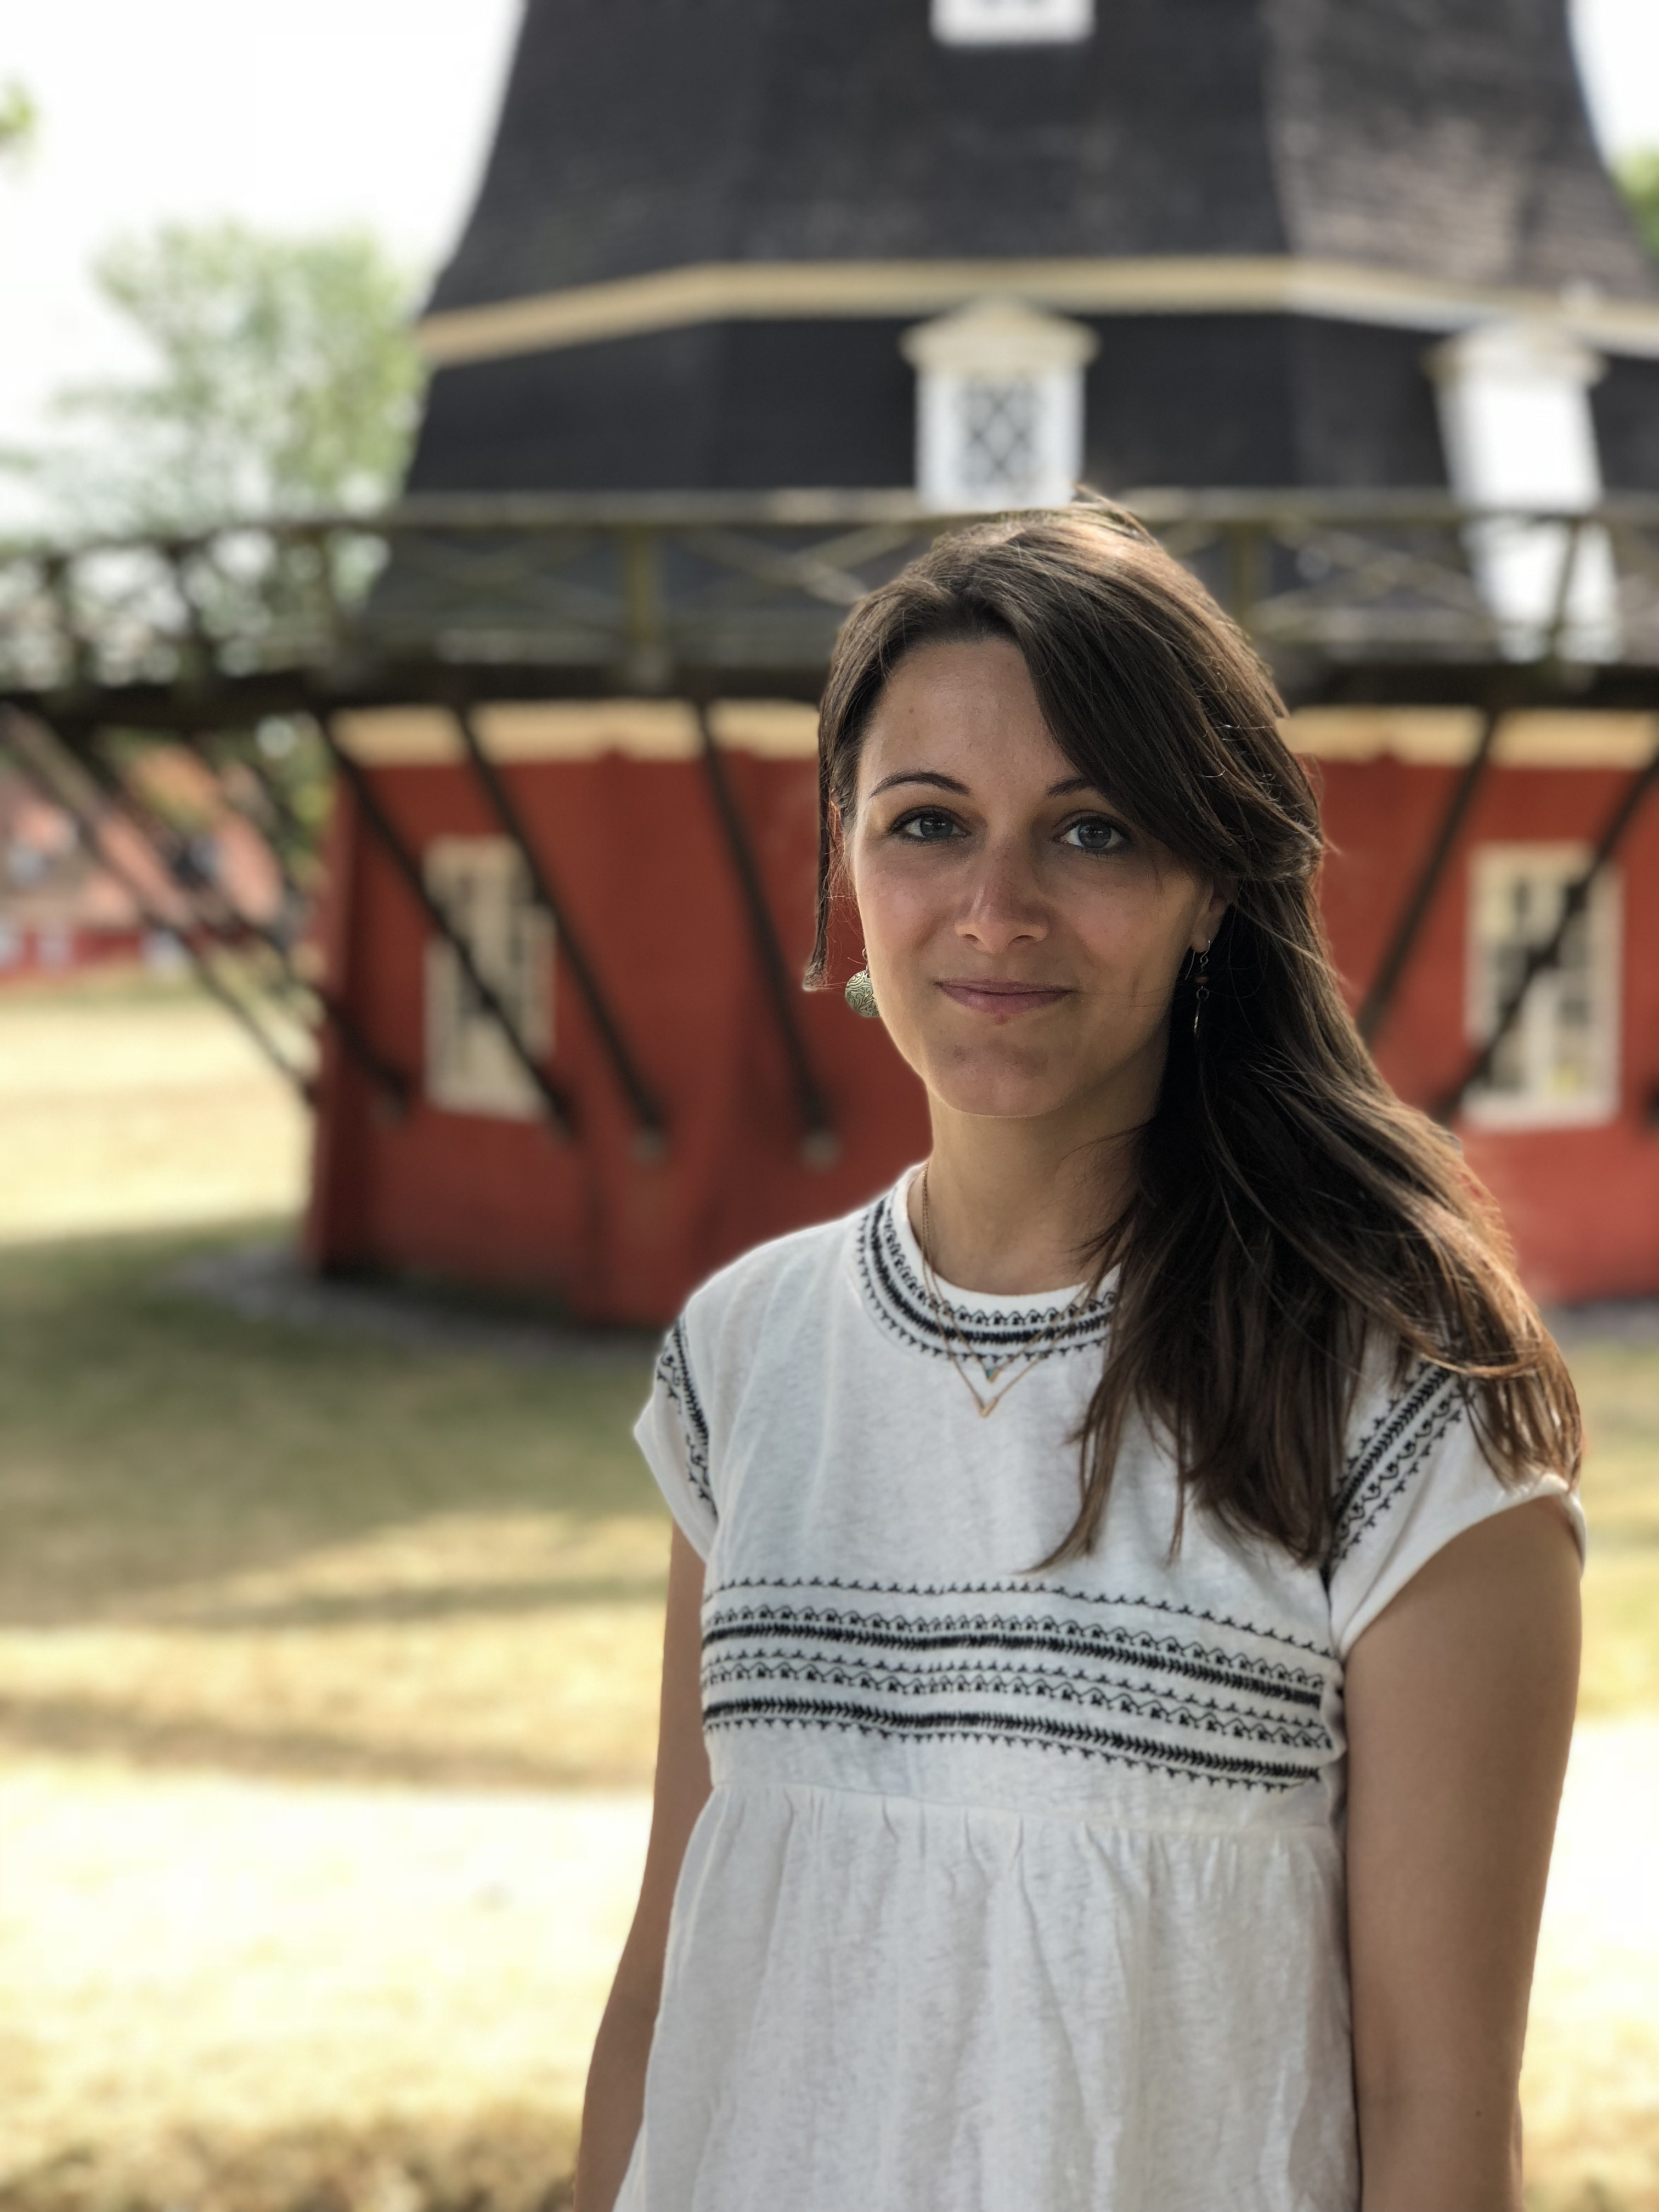
\includegraphics[width=0.95\columnwidth]{img/IMG_2838}
  \section{Skype}{\footnotesize{
    gessica.trivelli@gmail.com}}
  \section{Mail}{\footnotesize{
    \href{mailto:gessica.trivelli@gmail.com}{gessica.trivelli@gmail.com}}}
  \section{Angaben zur Person}\footnotesize{
    \textbf{Staatsangeh\"{o}rigkeit}: 
    Italienisch
    \textbf{Geburtsdatum}:
    14/04/1991
    \textbf{F\"{u}hrerschein}:
    B}
\end{aside}

\vspace{-10pt}
\section{Schul- und Berufsbildung}
\begin{entrylist}
  \entry
  {2017 - 2018}
  {Spezialisierung Kurs [EQF 7]}
  {\\Scuola Elementale di Arte Ostetrica, Florenz (Italien)}
  {\emph{
      Beckenbodengesundheit: Erziehung, Verhütung und Behandlung
      von Perineums Dysfunktion mit fachspezifischem Ansatz}. \\
    Ausbildung: 50 Creditpoints ECM – 194 Stunden.\\ 
    Diplomarbeit: \emph{Prolaps: jenseits des chirurgischen Eingriffs}.\\
  }

  \entry
  {2014 - 2017}
  {Master in Pflegewissenschaften und Geburtshilfe [EQF 7]}
  {\\Tor Vergata Universit\"{a}t, Rom (Italien)}
  {
    Summa cum Laude\\
    Masterarbeit: \emph{
      Erfahrungen und Einstellungen von
      M\"{u}ttern und Hebammen \"{u}ber verz\"{o}gerte Abnabelung
      und Nabelschnurblutstammzellenspende}  
    \\Forschungspraktikum: \emph{Istituto Superiore di Sanit\`{a}}, Rom (Italien).\\
  }
  
  \entry
  {2010 - 2014}
  {Studium der Geburtshilfe [EQF 6]}
  {\\Tor Vergata Universit\"{a}t, Rom (Italien)}
  {
    Summa cum Laude\\
    Bachelorarbeit: \emph{
      Untersuchung der Freiz\"{u}gigkeit und der antalgischen
      Positionen bei der Geburt: Bewertung der Ergebnisse von Mutter und Kind.}\\
    Praktikum in verschiedenen Krankenhäusern:
    \emph{Policlinico Tor Vergata (Rom, Italien)},
    \emph{Azienza Ospedaliera San Giovanni Addolorata (Rom, Italien)}, 
    \emph{Ospedale Fatebenefratelli San Giovanni Calibita (Rom, Italien)} e 
    \emph{Policlinico Casilino (Rom, Italien)}.\\
  }
  
  \entry
  {2005-2010}
  {Gymnasium mit Abiturabschluss [EQF 4]}
  {\\Liceo Scientifico "A. Gentili", Sarnano (Italien)}
  {\\}
\end{entrylist}

\vspace{-35pt}
\section{Berufserfahrung}
\begin{entrylist}
  %ia lecturer
  \entry
  {10/2019 -\\Heute}
  {Dozentin}
  {\\UniCamillus International Medical University, Rom (Italien)}
  {
    \emph{Maternity and Childcare Nursing},
    Gesundheits- und Krankenpflege Studium (Sprache: English) [1 ECTS].\\
    \emph{Scienze Infermieristiche Ostetrico-Ginecologiche II},
    Hebamme Studium (Sprache: Italienisch) [1 ECTS] \\
    \emph{Obstetrical and Gynaecological Nursing Sciences V},
    Hebamme Studium (Sprache: English) [2 ECTS] \\
    Website:
    \footnotesize{\url{https://www.unicamillus.org/it/personnel/trivelli-gessica-2}} .
  }

  %ia deutch midwife
  \entry
  {04/2019 -\\07/2020}
  {Hebamme}
  {\\Helios Klinik, Titisee Neustadt (Deutschland)}
  {Kreißsaal, Wochenbett Station.}

  %ia irish midwife
  \entry
  {07/2017 -\\11/2018}
  {Hebamme}
  {\\Coombe Women and Infants University Hospital, Dublin (Ireland)}
  {
    Gyn\"{a}kologische Praxis und Geburtshilfliche Sprechstunde.\\
    Pr\"{a}natalabtailung: Schwangerschaft und Risikoschwangerschaft Betreuung.\\
    Geburtshilfliche Ambulanz und Erste Hilfe.
  }
\end{entrylist}
%
%
\vspace{-10pt}
\begin{aside}
  \section{IT Skills}
  \textbf{Office}
\includegraphics[scale=0.40]{img/5stars.png}
  \textbf{Epi-Info}
\includegraphics[scale=0.40]{img/3stars.png}
  \textbf{Pubmed}
\includegraphics[scale=0.40]{img/5stars.png}
  \section{Technische F\"{a}higkeiten}\footnotesize{
    Probleml\"{o}sung
    ~
    Benutzung innovativer Lehrmodelle
    ~
    Erwachsenenbildung
    ~
    Planung, Implementation und Bewertung im klinischen, organisatorischen und p\"{a}dagogischen Bereich 
    ~
    Qualitative und quantitative Forschung im klinischen, organisatorischen und p\"{a}dagogischen Bereich
    ~
    Bewertung des Gesundheitsdienstes (z.b. Qualit\"{a}t, Zust\"{a}ndigkeit, Sicherheit, Kosten)}
  \section{Kommunikative F\"{a}higkeiten}\footnotesize{
    Counseling
    ~
    Empathie
    ~
    Aktives Zuh\"{o}ren}
\end{aside}


\section{Kursen und Zertificazionen}
\begin{entrylist}
  \entry
    {2020}
    {Resolving Shoulder Dystocia}
    {\\Spinning Babies - ACNM and MEAC approved (online course)}
    {3-Stunden- Kurs}
  \entry
    {2019}
    {TELC Zertifikat - B2}
    {\\TELC Deutsch}
    {\vspace{-10pt}}
  \entry
    {2018}
    {BLS provider - American Heart Association}
    {\\Center for Midwifery Education, Dublin (Ireland) - Irish Heart Foundation}
    {\vspace{-10pt}}
  \entry
    {2018}
    {K2MS Perinatal Training Programme (PTP)}
    {\\K2MS, Dublin (Ireland)}
    {Fetal monitoring and maternity crisis management training}
  \entry
    {2018}
    {Breastfeeding Refresher Programme}
    {\\Center for Midwifery Education, Dublin (Ireland)}
    {\vspace{-10pt}}
  \entry
    {2018}
    {Diabetes in Pregnancy Update}
    {\\Center for Midwifery Education, Dublin (Ireland)}
    {\vspace{-10pt}}
  \entry
    {2018}
    {Preceptorship Programme for Midwives and Nurses}
    {\\Center for Midwifery Education, Dublin (Ireland)}
    {\vspace{-10pt}}
  \entry
    {2018}
    {Water Immersion for Labour and Birth}
    {\\Center for Midwifery Education, Dublin (Ireland)}
    {\vspace{-10pt}}
  \entry
    {2017}
    {Haemovigilance and Infection Control}
    {\\Center for Midwifery Education, Dublin (Ireland)}
    {\vspace{-10pt}}
  \entry
    {2016}
    {Notf\"{a}lle der Geburt}
    {\\CreAttivaMente Ostetriche, Rom (Italien)}
    {16-Stunden- Kurs.}
  \entry
    {2015}
    {Fortgeschrittene Kompetenzen \"{u}ber Stillen Unterst\"{u}tzung.}
    {\\CreAttivaMente Ostetriche, Rom (Italien)}
    {16-Stunden- Kurs.}
  \entry
    {2014}
    {Stillen: Counseling und praktischer Kurs WHO-UNICEF Modell}
    {\\Tor Vergata Universit\"{a}t, Rom (Italien)}
    {40-Stunden- Kurs.}
\end{entrylist}

\newpage
\section{Sprachkenntnisse}
\begin{table*}[!h]
  \centering
  \renewcommand{\arraystretch}{1.45}
  \begin{tabular}{ p{3cm} p{3cm} p{3cm} p{3cm} }
    \hline
    & \textbf{Schreiben}       & \textbf{Sprechen} & \textbf{Verstehen}  \\     \hline
    \textbf{Italienisch:}      & \multicolumn{3}{c}{Muttersprache}       \\
    \textbf{Englisch:}         & C1 & C1 & C1                            \\ 
    \textbf{Deutsch:}          & B2 & B2 & B2                            \\ 
    \textbf{Franz\"{o}sisch:}  & A1 & A1 & A2                            \\    \hline
  \end{tabular}
\end{table*}

\section{Anerkennungen}
\begin{entrylist}
  \entry
    {2016}
    {Tutoratsstipendium}
    {\\Tor Vergata Universit\"{a}t, Rom (Italien)}
    {250 Uhr}
  \entry
    {2013}
    {Zusammenarbeitsstipendium}
    {\\Tor Vergata Universit\"{a}t, Rom (Italien)}
    {150 Uhr}
\end{entrylist}

\vspace{-10pt}
\section{Berufliche Anerkennung}
\begin{itemize}
  \item[--] Italien: \emph{Ordine delle Ostetriche di Roma} - n°2640 (Eintragungsdatum 25/02/2015)
  \item[--] Deutschland - Baden-W\"{u}rttemberg: \emph{Regierungspr\"{a}sidium Stuttgart} (Eintragungsdatum 11/07/2019)
  \item[--] Die Schweiz: SRK Anerkennung - NAREG n° HEB20201165 (Eintragungsdatum 28/04/2020)
\end{itemize}

%% \vspace{75pt}
%% \footnotesize La sottoscritta è a conoscenza che, ai sensi dell’art. 26 della legge 
%% 15/68, le dichiarazioni mendaci, la falsità negli atti e l’uso di
%% atti falsi sono puniti ai sensi del codice penale e delle leggi speciali. Inoltre, il 
%% sottoscritto autorizza al trattamento dei dati
%% personali, secondo quanto previsto dalla Legge 675/96 del 31 dicembre 1996.

\vspace{75pt}
\begin{flushleft}
\large\emph{Rom, 22 Juli 2020}
\end{flushleft}
\begin{flushright}
\large\emph{Gessica Trivelli}
\end{flushright}

\end{document}

